\section{Image processing and information extraction}\label{sec:improc}

\subsection{Simple calculus with channels}\label{ssec:calculus}

todo.

\subsection{Classification}\label{ssec:classification}

The aim of the new SVM classification framework is to provide a supervised pixel-wise classification chain based on learning from multiple images. It supports huge images through streaming and multi-threading.
The classification chain will perform a SVM training step based on the intensities of each pixel as features. Please note that the images will have the same number of bands to be comparable.

\subsubsection{Statistics estimation}
In order to make these features comparable between each images, the first step is to estimate the statistic of the group of input images. These statistics will be used to center and reduce the intensities (mean of 0, std dev of 1) of samples based on the vector data produced by the user. To do so, the \textbf{otbEstimateImagesStatistics} tool can be used :

\begin{verbatim}
otbEstimateImagesStatistics-cli -in  list_of_input_images 
                                -out statistics.xml
\end{verbatim}

This tool will compute the mean of each band, compute the standard deviation based on pooled variance of each band and finally exporting them to an XML file.

The features statistics XML file will be an input of the following tools. 

\subsubsection{Building a training data set}

The chain is supervised : one has to build a training set with positive examples of different objects of interest. This can be done with the Vectorization Monteverdi module (Fig.\ref{fig:vectoModuleDataSetCreation}), by building a VectorData containing polygons centered on occurrences of the different objects of interest. This operation will be reproduce on each images used as input of the training function.

Please note that the positive examples in the vector data should have a Class field with a label higher than 1 and coherent in each different images. 

\begin{figure}
  \center
  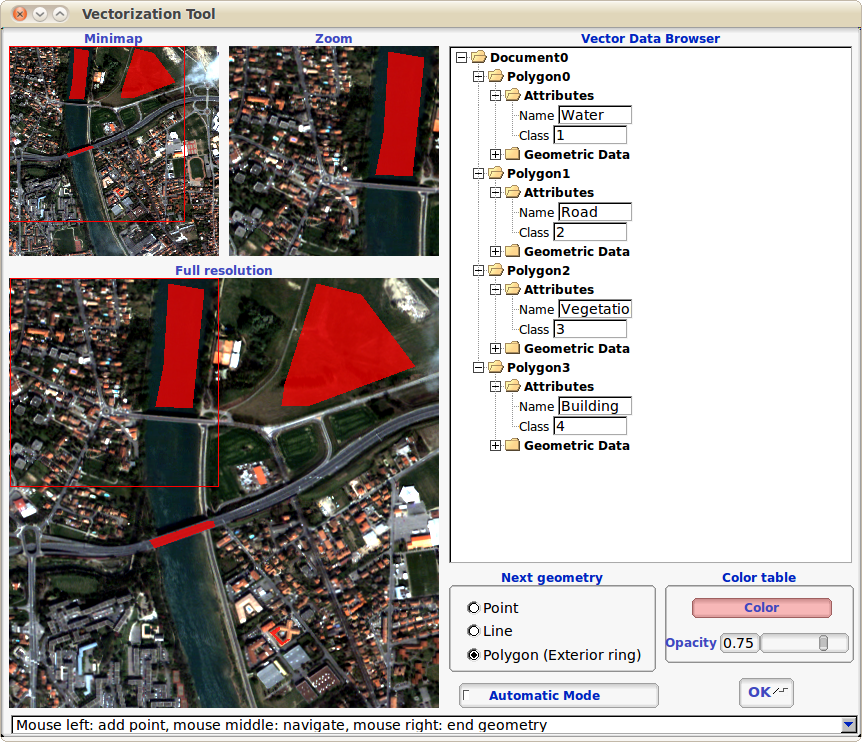
\includegraphics[width=1\textwidth]{../Art/MonteverdiImages/monteverdi_vectorization_module_for_classification.png}
  \itkcaption[GUI of the vectorization module with data for classification chain]{A training data set builded with the vectorization monteverdi module.}
  \label{fig:vectoModuleDataSetCreation}
\end{figure}

You can generate the vector data set with QGIS software for example. The OTB-applications should be able to transform the vectordata into the corrdinate system of the image. 

\subsubsection{Training data set}

Once images statistics have been estimated, the learning scheme is the following:
\begin{enumerate}
  \item For each of the input images:
  \begin{enumerate}
    \item Read the region of interest (ROI) inside the shapefile,
    \item Generate validation and training data within the ROI,
    \item Add the vectors respectively to the training samples set and the validation samples set.
  \end{enumerate}
  \item Increase the size of the training samples set and balance it by generating new noisy samples from the previous ones,
  \item SVM learn with this training set
  \item Estimate performances of the SVM classifier on the validation samples set (confusion matrix, precision, recall).
\end{enumerate}

These steps can be performed by the \textbf{otbTrainImagesClassifier} program using the following:

\begin{verbatim}
otbTrainImagesClassifier-cli -is  images_statistics.xml 
                             -in  list_of_input_images 
                             -vd  list_of_positive_examples_shapefiles
                             -out model.svm
                             -b
\end{verbatim}

Some options are available:
\begin{itemize}
\item -dem \textit{a DEM repository to keep accurate reprojection of vectordata}
\item -m   \textit{margin value}
\item -k   \textit{svm kernel (0 = LINEAR (default), 1 = RBF,  2 = POLY, 3 = SIGMOID) }
\item -opt \textit{use svm parameters optimization}
\item -mt  \textit{maximum training samples size} 
\item -mv  \textit{maximum validation samples size}
\item -vrt \textit{ratio validation training}
\end{itemize}

\subsubsection{Validate the classification model}
It is also possible to estimate the performance of the svm model with a new set of validation samples and another image with the following application.
It will compute the global confusion matrix and precision, recall and F-score of each class based on the \href{http://www.orfeo-toolbox.org/doxygen-current/classotb_1_1ConfusionMatrixCalculator.html}{ConfusionMatrixCalculator} class.
It is done by \textbf{otbValidateImagesClassifier}:

\begin{verbatim}
otbValidateImagesClassifier-cli -is  images_statistics.xml
                                -svm model.svm
                                -in  input_image
                                -vd  list_of_positive_examples_shapefiles
\end{verbatim}

You can save these results with the option -out output filename. You also can set a DEM repository (-dem) to keep accurate reprojection of vectordata.

\subsubsection{Using the classification model} 
Once the classifier has been trained, one can apply the model to classify pixel inside defined classes on a new image using the \textbf{otbImageSVMClassifier} tool:

\begin{verbatim}
 otbImageSVMClassifier-cli -is  images_statistics.xml
                           -svm model.svm 
                           -in  input_image
                           -out labeled_image
\end{verbatim}

You can set an input mask to restricted the classification to the mask area with value \textgreater 0.

\subsubsection{Fancy classification results}

In order to get an RGB classification map instead of greylevel labels, one can use the \textbf{otbLabeledImageColorMapping} tool. This tool will replace each label with an 8-bits RGB color specificied in a mapping file. The mapping file should look like this :

\begin{verbatim}
# Lines beginning with a # are ignored
1 255 0 0
\end{verbatim}

In the previous example, 1 is the label and 255 0 0 is a RGB color (this one will be rendered as red). To use the mapping tool, enter the following :

\begin{verbatim}
otbLabeledImageColorMapping-cli -in  labeled_image 
                                -out color_image
                                -ct  mapping_file
\end{verbatim}

\subsubsection{Example}
We take 4 classes: water, roads, vegetation and buildings with red roof.
Data are available in the OTB-Data \href{http://hg.orfeo-toolbox.org/OTB-Data/file/0fed8f4f035c/Input/Classification}{repository} and this image is produced with the commands inside this \href{http://hg.orfeo-toolbox.org/OTB-Applications/file/3ce975605013/Testing/Classification/CMakeLists.txt}{file}. 

\begin{figure}[!h]
  \center
  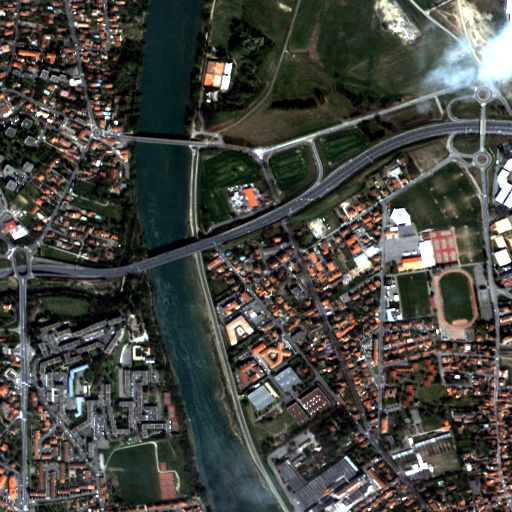
\includegraphics[width=0.3\textwidth]{../Art/MonteverdiImages/classification_chain_inputimage.jpg}
  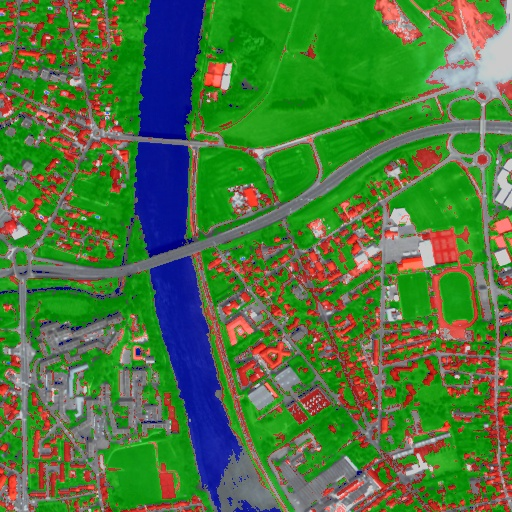
\includegraphics[width=0.3\textwidth]{../Art/MonteverdiImages/classification_chain_fancyclassif_fusion.jpg}
  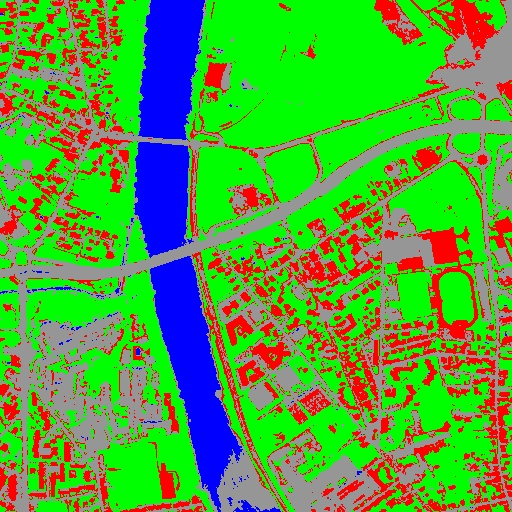
\includegraphics[width=0.3\textwidth]{../Art/MonteverdiImages/classification_chain_fancyclassif.jpg}}
  \itkcaption[ExampleSVMCalssif]{From left to right: Original image, result image with fusion (with monteverdi viewer) of original image and fancy classification and input image with fancy color classification from labeled image.}
  \label{fig:MeanShiftVectorImageFilter}
\end{figure}



\subsection{Segmentation}\label{ssec:segmentation}

todo.

\subsection{Change detection}\label{ssec:changedetection}

todo.

\subsection{Object-based image analysis}\label{ssec:obia}

todo.

